\documentclass[
  bibliography=totoc,     % Literatur im Inhaltsverzeichnis
  captions=tableheading,  % Tabellenüberschriften
  titlepage=firstiscover, % Titelseite ist Deckblatt
]{scrartcl}

% Paket float verbessern
\usepackage{scrhack}

% Warnung, falls nochmal kompiliert werden muss
\usepackage[aux]{rerunfilecheck}

% unverzichtbare Mathe-Befehle
\usepackage{amsmath}
% viele Mathe-Symbole
\usepackage{amssymb}
% Erweiterungen für amsmath
\usepackage{mathtools}

% Fonteinstellungen
\usepackage{fontspec}
% Latin Modern Fonts werden automatisch geladen
% Alternativ zum Beispiel:
%\setromanfont{Libertinus Serif}
%\setsansfont{Libertinus Sans}
%\setmonofont{Libertinus Mono}

% Wenn man andere Schriftarten gesetzt hat,
% sollte man das Seiten-Layout neu berechnen lassen
\recalctypearea{}

% deutsche Spracheinstellungen
\usepackage[ngerman]{babel}


\usepackage[
  math-style=ISO,    % ┐
  bold-style=ISO,    % │
  sans-style=italic, % │ ISO-Standard folgen
  nabla=upright,     % │
  partial=upright,   % │
  mathrm=sym,        % ┘
  warnings-off={           % ┐
    mathtools-colon,       % │ unnötige Warnungen ausschalten
    mathtools-overbracket, % │
  },                       % ┘
]{unicode-math}

% traditionelle Fonts für Mathematik
\setmathfont{Latin Modern Math}
% Alternativ zum Beispiel:
%\setmathfont{Libertinus Math}

\setmathfont{XITS Math}[range={scr, bfscr}]
\setmathfont{XITS Math}[range={cal, bfcal}, StylisticSet=1]

% Zahlen und Einheiten
\usepackage[
  locale=DE,                   % deutsche Einstellungen
  separate-uncertainty=true,   % immer Unsicherheit mit \pm
  per-mode=symbol-or-fraction, % / in inline math, fraction in display math
]{siunitx}

% chemische Formeln
\usepackage[
  version=4,
  math-greek=default, % ┐ mit unicode-math zusammenarbeiten
  text-greek=default, % ┘
]{mhchem}

% richtige Anführungszeichen
\usepackage[autostyle]{csquotes}

% schöne Brüche im Text
\usepackage{xfrac}

% Standardplatzierung für Floats einstellen
\usepackage{float}
\floatplacement{figure}{htbp}
\floatplacement{table}{htbp}

% Floats innerhalb einer Section halten
\usepackage[
  section, % Floats innerhalb der Section halten
  below,   % unterhalb der Section aber auf der selben Seite ist ok
]{placeins}

% Seite drehen für breite Tabellen: landscape Umgebung
\usepackage{pdflscape}

% Captions schöner machen.
\usepackage[
  labelfont=bf,        % Tabelle x: Abbildung y: ist jetzt fett
  font=small,          % Schrift etwas kleiner als Dokument
  width=0.9\textwidth, % maximale Breite einer Caption schmaler
]{caption}
% subfigure, subtable, subref
\usepackage{subcaption}

% Grafiken können eingebunden werden
\usepackage{graphicx}

% schöne Tabellen
\usepackage{tabularray}
\UseTblrLibrary{booktabs, siunitx}

% Verbesserungen am Schriftbild
\usepackage{microtype}

% Literaturverzeichnis
\usepackage[
  backend=biber,
]{biblatex}
% Quellendatenbank
\addbibresource{lit.bib}
\addbibresource{programme.bib}

% Hyperlinks im Dokument
\usepackage[
  german,
  unicode,        % Unicode in PDF-Attributen erlauben
  pdfusetitle,    % Titel, Autoren und Datum als PDF-Attribute
  pdfcreator={},  % ┐ PDF-Attribute säubern
  pdfproducer={}, % ┘
]{hyperref}
% erweiterte Bookmarks im PDF
\usepackage{bookmark}

% Trennung von Wörtern mit Strichen
\usepackage[shortcuts]{extdash}

\author{%
  Vincent Wirsdörfer\\%
  \href{mailto:vincent.wirsdoerfer@udo.edu}{authorA@udo.edu}%
  \and%
  Joris Daus\\%
  \href{mailto:joris.daus@udo.edu}{authorB@udo.edu}%
}
\publishers{TU Dortmund – Fakultät Physik}


\begin{document}
\section{Auswertung}
\label{sec:Auswertung}

Die Spannungamplitude der Referenzspannung kann variiert werden. Bei der Oszillatorspannung, also der Signalspannung 
ist die Amplitude konstant und beträgt $U=3.2 \, \unit{\volt}$.\\
Die im Lock-In-Verstärker gemischten Spannungen, werden für eine Phasenverschiebung 
$\varphi= 0°,\, 90°,\, 180°,\, 270° \ \text{und} \ 315°$ abfotografiert. Die Phasenverschiebung beschreibt dabei die 
Phase, welche zwischen der Referenz- und der Signalspannung liegt. Die Ausgangsspannung des Verstärkers besitzt dann 
folgende Formen:

\begin{figure}
    \begin{subfigure}{0.48\textwidth}
        \centering
        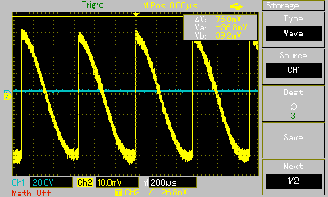
\includegraphics{Oszilloskop_0.pdf}
        \caption{Phasenverschiebung $\varphi = 0°$}
        \label{fig:0deg}
    \end{subfigure}
    \hfill
    \begin{subfigure}{0.48\textwidth}
        \centering
        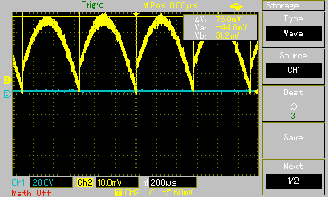
\includegraphics{Oszilloskop_90.pdf}
        \caption{Phasenverschiebung $\varphi = 90°$}
        \label{fig:90deg}
    \end{subfigure}
    \hfill
    \begin{subfigure}{0.48\textwidth}
        \centering
        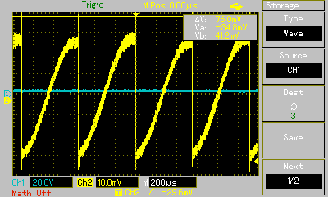
\includegraphics{Oszilloskop_180.pdf}
        \caption{Phasenverschiebung $\varphi = 180°$}
        \label{fig:180deg}
    \end{subfigure}
    \hfill
    \begin{subfigure}{0.48\textwidth}
        \centering
        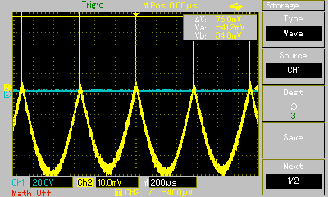
\includegraphics{Oszilloskop_270.pdf}
        \caption{Phasenverschiebung $\varphi = 270°$}
        \label{fig:270deg}
    \end{subfigure}
    \hfill
    \begin{subfigure}{0.48\textwidth}
        \centering
        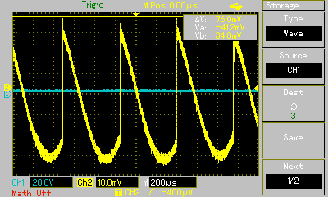
\includegraphics{Oszilloskop_315.pdf}
        \caption{Phasenverschiebung $\varphi = 315°$}
        \label{fig:315deg}
    \end{subfigure}    
\caption{Spannungsverläufe in Abhängigkeit der Phase zwischen Referenz und Signal.}
\end{figure}

\noindent
Die Abbildungen, zwischen denen jeweils $180°$ liegen sind an der x-Achse gespiegelt. Dies liegt an daran, dass die 
Referenzspannung immer genau das gleiche beziehungsweise immer genau das entgegengesetzte Vorzeichen wie die 
Signalspannung besitzt. So hat zum Beispiel die Referenzspannung in \autoref{fig:90deg} das gleiche Vorzeichen wie die 
Signalspannung, weshalb nur positive Komponenten existieren. So haben in \autoref{fig:180deg} haben Referenz- und 
Signalspannung genau entgegengesetzte Vorzeichen.
Gleiches lässt sich auch bei \autoref{fig:0deg} und \autoref{fig:180deg} beobachten.\\
\noindent
Im folgenden werden die Messdaten aud \autoref{tab:no_noise} und \autoref{tab:mit_noise} ausgewertet. Die gemessene 
Spannung wird gegen die eingestellte Phasenverschiebung aufgetragen. Über ein Pythonprogramm wird zu der 
theoretisch vorhergesagten Funktion \eqref{eqn:U_out} eine Kurve gefittet.

\begin{figure}[H]
    \includegraphics[width=\textwidth]{../build/no_noise.pdf}
    \caption{Nicht verrauschtes Signal.}
    \label{fig:fit_no_noise}
\end{figure}

\begin{figure}[H]
    \includegraphics[width=\textwidth]{../build/mit_noise.pdf}
    \caption{Verrauschtes Signal.}
    \label{fig:fit_mit_noise}
\end{figure}

\noindent
Zu sehen sind Wellen, die mithilfe der postulierten cosinus Welle beschrieben werden. 

\end{document}
